\documentclass[a4paper,10pt]{article}
\usepackage[utf8]{inputenc}
\usepackage{graphicx}
\usepackage{float}
\usepackage{comment}
\usepackage[ngerman]{babel}
\usepackage[pdfborder={0 0 0}]{hyperref}
\usepackage{lmodern,textcomp}
\usepackage{subfigure}

\title{
    183.289 VU Interface \& Interaction Design \\
    WS 2012 / 2013 \\
    Beispiel 3}
\author{
    Gruppe 5 \\ \\
    Jakob Gruber, 0203440, 033 534 \\
    Rene Pointner, 0526792, 033 532\\
    Mino Sharkhawy, 1025887, 033 534 \\
    Stefan Sietzen, 0372194, 033 532}

\begin{document}

\maketitle

\clearpage
\tableofcontents

\clearpage
\section{Umsetzung des Prototypen}

Der interaktive Prototyp (in diesem Dokument IP genannt) \emph{Finance Buddy} wurde mit Hilfe von Twitter
Bootstrap\footnote{\url{http://twitter.github.com/bootstrap/index.html}}
und jQuery-UI\footnote{\url{http://jqueryui.com/} und
\url{http://addyosmani.github.com/jquery-ui-bootstrap/}} in HTML5 realisiert.

Als Vorlage wurde der angepasste Low-Fidelity-Prototype der zweiten Aufgabe von Interface \&
Interaction Design (in diesem Dokument LFP genannt) verwendet. Es wurden dabei einzelne Screens nacheinander als
entsprechende HTML Seiten erstellt. Kleinere, von einander getrennte Screens mit
wenig gemeinsamen Elementen (wie zum Beispiel Login, Registration, und Password Recovery)
sind als separate HTML Seiten gehalten worden, w\"ahrend der eigentliche Hauptteil
der Applikation in einer einzigen Seite realisiert wurde.

Der Gedanke dahinert war vor allem Arbeitsersparnis. Durch viele gemeinsame Elemente (unter
anderem die gesamte Leiste auf der linken Seite des Bildschirms) h\"atte sich der
Arbeitsaufwand vervielfacht wenn die jeweiligen Untersektionen (\emph{Expenses},
\emph{Recurring Expenses}, \emph{Graphs}, etc\ldots) separate HTML Seiten waeren.

Die L\"osung st\"utzt sich somit auf JavaScript um UI Elemente dynamisch ein- und
auszublenden oder anderwertig zu ver\"andern. Zum Beispiel wird bei einem Click auf
den \emph{Recurring Expenses} Entrag die passende rechte Seite des Screens eingeblendet,
die linke Seite wird mit den richtigen Elementen bef\"ullt, und der Navigationseintrag
wird als aktiv markiert.

\subsection{Abweichungen vom urspr\"unglichen Konzept}

\begin{comment}
Beschreiben Sie kurz die Umsetzung Ihres interaktiven Prototypen. Insbesondere sollen darin folgende Fragen beantwortet werden (jeweils soweit sie auf Ihren Entwicklungsprozess anwendbar sind):

Welche Änderungen waren bei der Umsetzung des interaktiven Prototypen im Vergleich zu Ihrem ursprünglichen Konzept notwendig und weshalb (technische Einschränkungen, Komplexität, ...)?

Welche Aspekte waren in Ihrem ursprünglichen Konzept unterspezifiziert und mussten bei der Umsetzung konkretisiert werden?

Auf welche Schwächen und Probleme in Ihrem Konzept sind Sie bei der Umsetzung des interaktiven Prototypen aufmerksam geworden?


Illustrieren Sie Abweichungen anhand von Wireframes aus Ihrem ursprünglichen Konzept und stellen Sie sie Screenshots aus dem interaktiven Prototypen gegenüber. Heben Sie ggf. spezifische Details graphisch oder in Form von Anmerkungen hervor.
\end{comment}

\subsubsection{Login}

% TODO: Side-by-side comparison images

Der Login Screen ist von den Funktionen her identisch zum LFP. Es wurden mehrere
kleinere \"Anderungen an dem Look \& Feel vorgenommen: wichtige Elemente wie der
Sign In Button wurden durch Typographie und Farbgestaltung hervorgehoben, und das Layout
ist nun im IP sinnvoller gestaltet.

Bei falschen Eingaben (zum Beispiel einem leeren Username Feld) wird dem Benutzer
deutlicher Feedback in Form eines roten Alerts angezeigt.

\subsubsection{Password Recovery}

\begin{figure}
\centering
\mbox{
    \subfigure{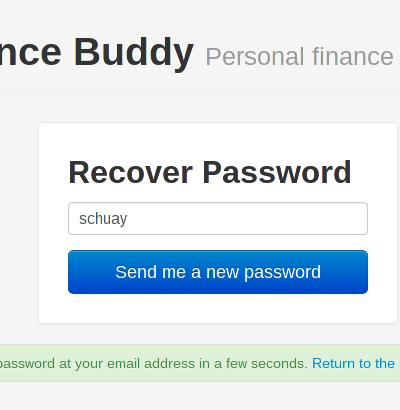
\includegraphics[width=0.5\textwidth]{password-recovery-ip}}\quad
    \subfigure{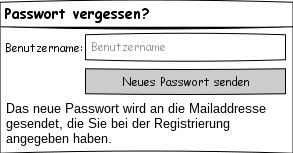
\includegraphics[width=0.5\textwidth]{password-recovery-lfp}}
}
\caption{Password Recovery} \label{fig:password-recovery}
\end{figure}

Das Layout ist im IP um einiges simpler gestaltet als im LFP. Wichtige Elemente
sind hervorgehoben, and Zusatzinfos zu n\"achsten Schritten nach der ausf\"ullen
des Formulars werden erst angezeigt wenn sie relevant sind.


\clearpage
\subsection{Einschränkungen des interaktiven Prototypen}

\begin{comment}
Welche Aspekte konnten in Ihrem interaktiven Prototypen nur unvollständig umgesetzt werden (z.B. weil der Umsetzungsaufwand zu hoch wäre)? Beschreiben Sie eventuelle Kompromisslösungen ausreichend genau, dass Ihre geplante und beabsichtigte Funktionsweise für den Leser klar verständlich und nachvollziehbar ist.
\end{comment}

\begin{itemize}
    \item Registrierung, Login und Password Recovery testen die Eingaben zwar auf
            Korrektheit, haben aber keine echte Nutzerdatenbank. Der Login akzeptiert
            jede Benutzername/Passwort-Kombination.
    \item Das Sortieren nach Spalten unter \glqq Expenses\grqq, \glqq
            Recurring Expenses\grqq\space und dem Suchergebnis ist mit dem Prototypen
            nicht m\"oglich.
    \item Der \glqq Add New Recurring Expense\grqq\space Dialog führt
            Fehler\"uberprüfung durch, es ist aber nicht m\"oglich einen neuen
            Eintrag hinzuzuf\"ugen.
    \item Die \glqq Edit\grqq\space und \glqq Remove\grqq\space Buttons unter \glqq
            Recurring Expenses\grqq\space funktionieren wegen des hohen Aufwands
            nicht. Der \glqq Edit\grqq\space Dialog sieht aus wie der zum
            Hinzuf\"ugen und wird unter der entsprechenden Zeile angezeigt.
    \item Die Suche und erweiterte Suche liefern keine echten Ergebnisse sondern nur
            eine statische Seite.
    \item Die Buttons \glqq August 2012\grqq, \glqq July 2012\grqq\space und \glqq
            June 2012\grqq\space unter \glqq Expenses\grqq\space haben keine
            Funktion.
    \item Die Einstellungen unter \glqq Settings\grqq\space wirken sich nicht auf
            andere Anzeigen aus und gehen nachdem die Seite neu geladen wurde
            verloren.
    \item Unabh\"angig davon welcher Zeitraum oder welche Kategorie unter \glqq
            Graphs\grqq\space ausgew\"ahlt wurde, gibt es nur zwei Graphen als
            Bilder.
    \item Unter \glqq Expenses\grqq\space kann man mit dem \glqq Add New
            Expense\grqq\space Dialog genau einen neuen Eintrag hinzuf\"ugen indem
            man nach Eingabe der Daten auf \glqq Submit\grqq\space klickt. \glqq
            Submit and Continue\grqq\space f\"ugt keinen Datensatz hinzu. Der neue
            Eintrag wird \"uber GET-Parameter gesichert und erscheint im Suchergebnis
            und unter \glqq Expenses\grqq\space jeweils an erster Stelle. F\"ur
            diesen und nur diesen Eintrag funktionieren die \glqq Edit\grqq\space und
            \glqq Remove\grqq\space Buttons.
    \item Wenn ein funktionierender \glqq Submit\grqq\space Button gedr\"uckt wird
            und die Seite neu geladen wird landet man wieder unter \glqq
            Expenses\grqq\space auf der Seite f\"ur Oktober 2012. Tats\"achlich
            sollte man aber auf der selben Seite bleiben. Das ist aber relativ
            schwierig und komplex umzusetzen.
    \item Beim Eingeben einer Kategorie (\glqq Category\grqq-Feld) sollten nicht nur
            Vorschl\"age angezeigt werden, sondern auch bereits angelegte Kategorien
            \"uber ein Drop-Down-Men\"u ausgew\"ahlt werden k\"onnen. Das war aber
            mit den gegebenen Mitteln zu aufw\"andig.
    \item Der Beispieleintrag, den man wie oben erkl\"art anlegen kann, ver\"andert
            weder die Grafiken unter \glqq Graphs\grqq, noch den Balken und die Daten
            in der Zusammenfassung links unten.
\end{itemize}

\end{document}
